\documentclass[11pt]{elegantbook}

\title{\LaTeX{} codes}
\subtitle{\LaTeX{} Template}

\author{Zhutao Sheng}
\date{2022}

\extrainfo{Victory won\rq t come to us unless we go to it. }

\cover{cover.jpg}

% modify the color in the middle of titlepage
\definecolor{customcolor}{RGB}{32,178,170}
\colorlet{coverlinecolor}{customcolor}

\begin{document}

\maketitle

\frontmatter
\tableofcontents

\mainmatter

\chapter{Elegant\LaTeX{} Templates}
Elegant\LaTeX{} codes

\section{title}
The corresponding code is: 
\begin{lstlisting}
\title{\LaTeX{} codes}
\maketitle
\end{lstlisting}


\section{references}
The corresponding code is: 
\begin{lstlisting}
\addbibresource{references.bib}
\cite{bibid}
\printbibliography
\end{lstlisting}

\section{Character}
And symbol Z \& S

\section{Figure}


\begin{figure}[htbp]
	\centering
	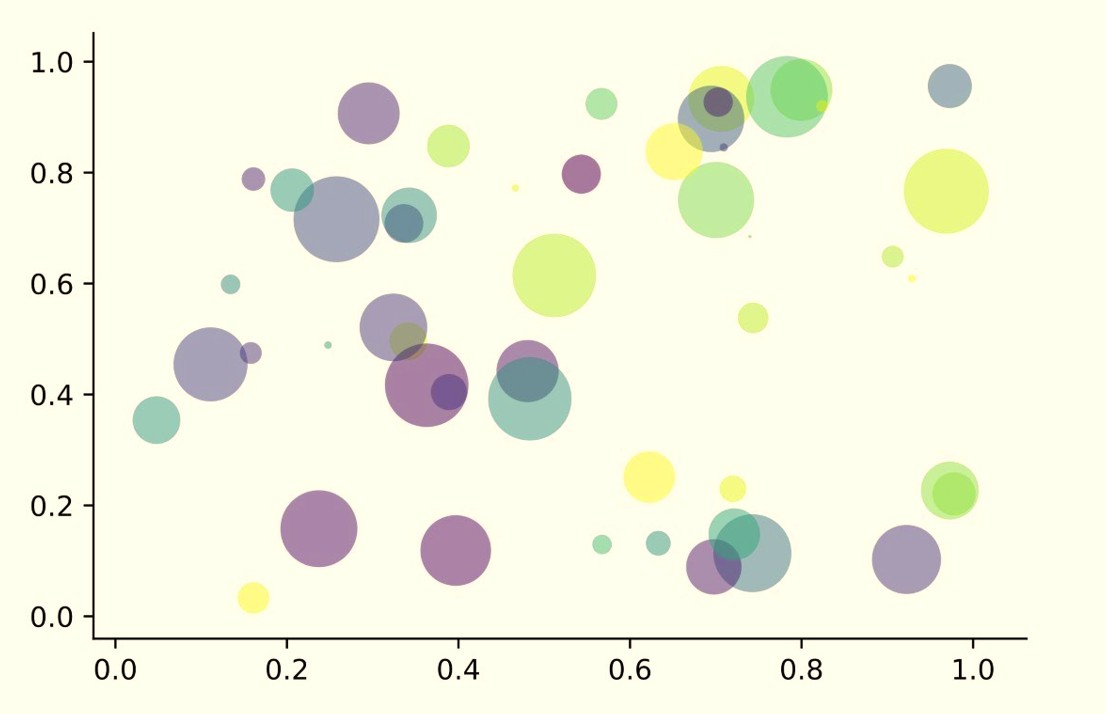
\includegraphics[width=0.6\textwidth]{figure/scatter.jpg}
	\caption{Matplotlib: Scatter Plot Example\label{fig:scatter}}
\end{figure}
% only two parameters can be set image	\centering 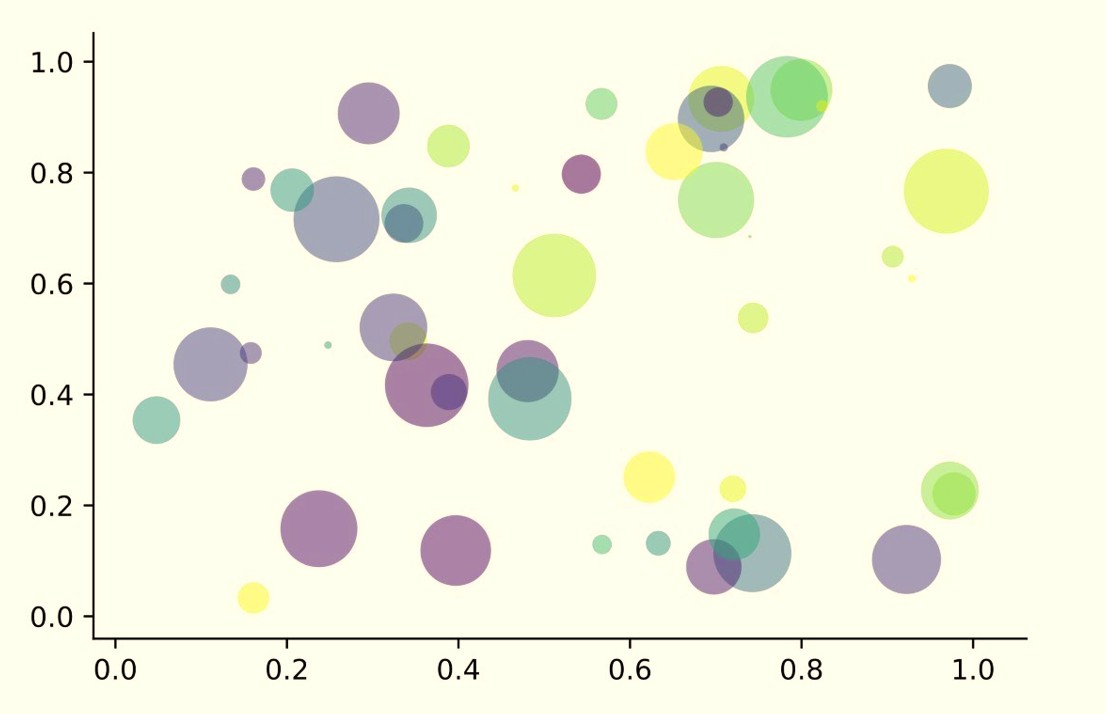
\includegraphics{figure/scatter.jpg}
The corresponding code is: 
\begin{lstlisting}
	\begin{figure}[htbp]
		\centering
		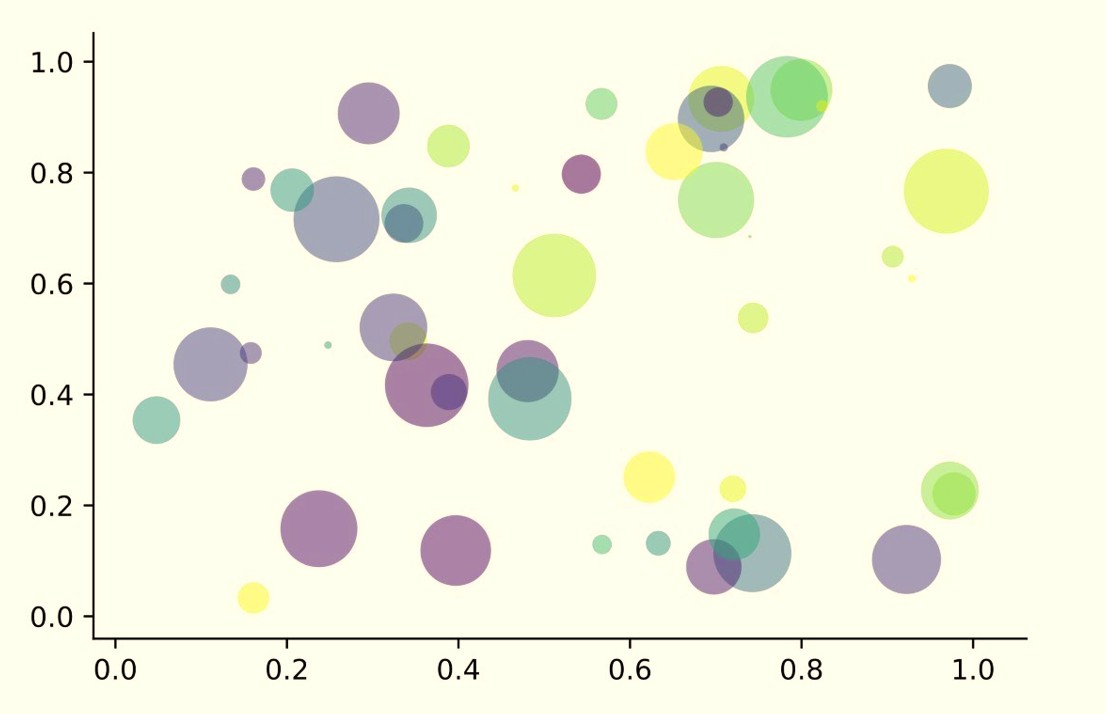
\includegraphics[width=0.6\textwidth]{figure/scatter.jpg}
		\caption{Matplotlib: Scatter Plot Example\label{fig:scatter}}
	\end{figure}
\end{lstlisting}

% the parameter can be changed as: width=\textwidth,  this is larger width = page scale.

\begin{figure}[ht]
	\begin{minipage}[b]{0.45\linewidth}
		\centering
		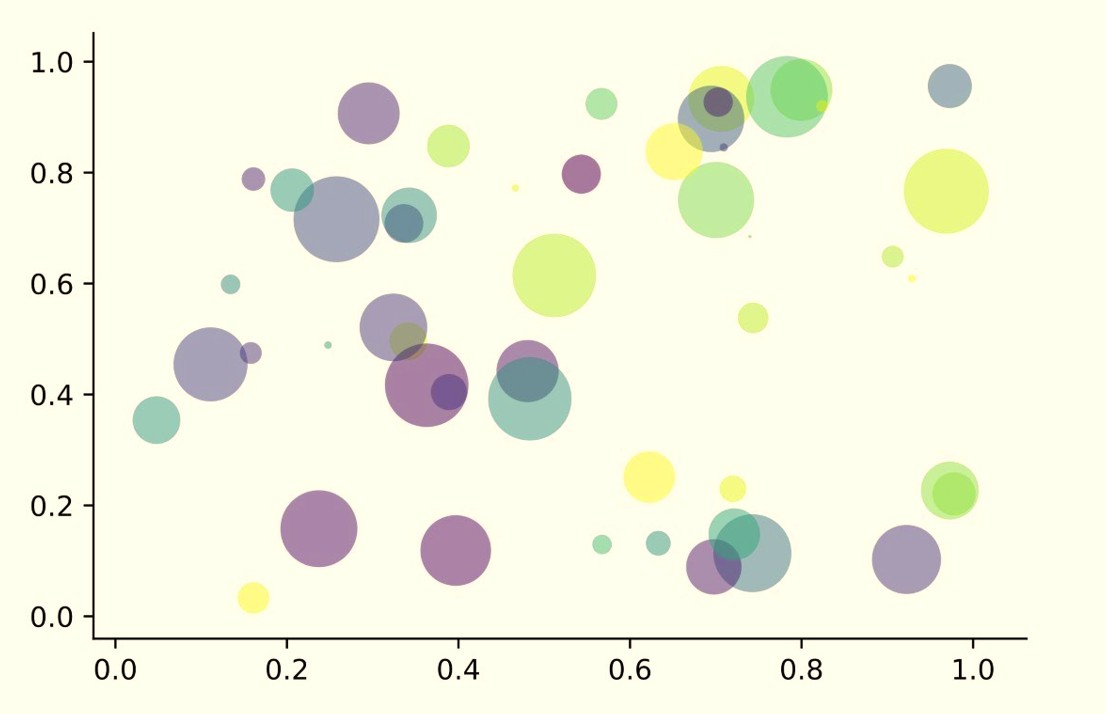
\includegraphics[width=\textwidth]{figure/scatter.jpg}
		\caption{South American coati}
		\label{fig:nasua}
	\end{minipage}
	\hspace{0.5cm}
	\begin{minipage}[b]{0.45\linewidth}
		\centering
		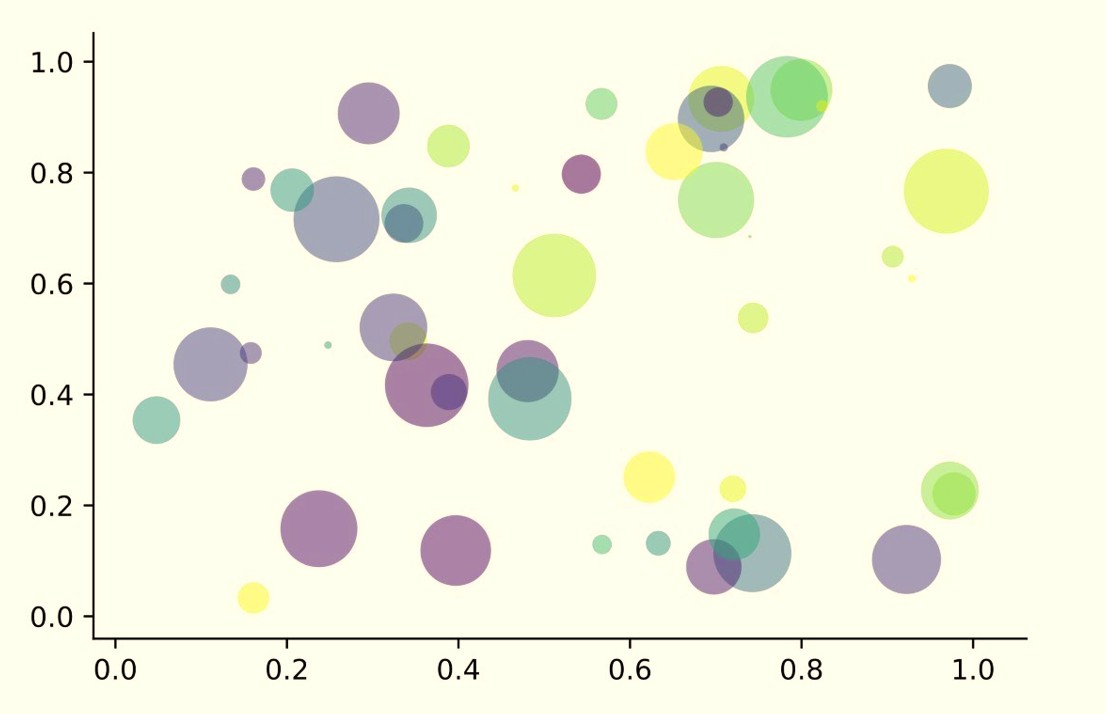
\includegraphics[width=\textwidth]{figure/scatter.jpg}
		\caption{Brown bear}
		\label{fig:Ursus-arctos}
	\end{minipage}
\end{figure}
The double image in one row /side-by-side corresponding code is: 
\begin{lstlisting}
\begin{figure}[ht]
	\begin{minipage}[b]{0.45\linewidth}
		\centering
		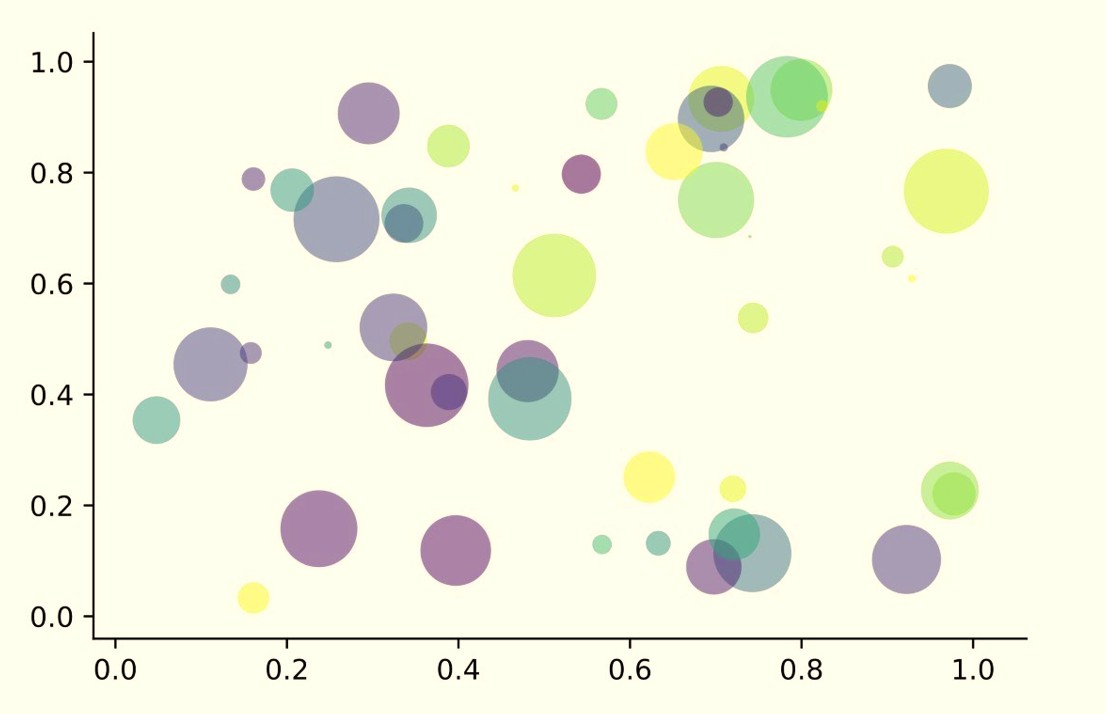
\includegraphics[width=\textwidth]{figure/scatter.jpg}
		\caption{figure 1}
		\label{fig:nasua}
	\end{minipage}
	\hspace{0.5cm}
	\begin{minipage}[b]{0.45\linewidth}
		\centering
		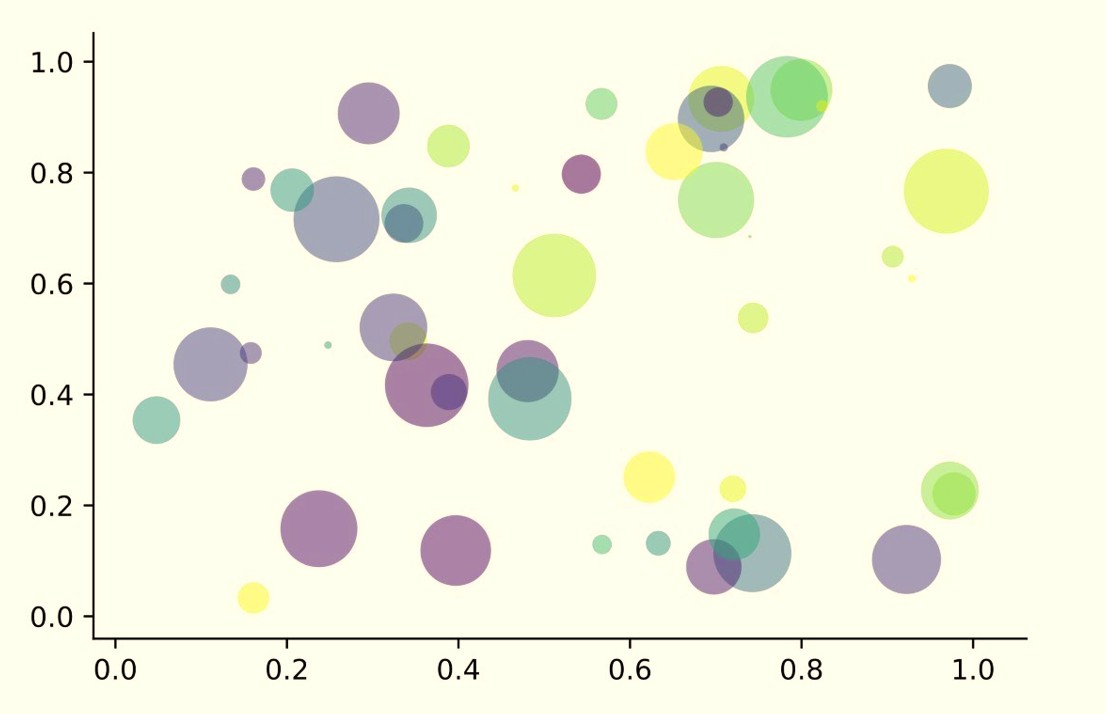
\includegraphics[width=\textwidth]{figure/scatter.jpg}
		\caption{figure 2}
		\label{fig:Ursus-arctos}
	\end{minipage}
\end{figure}
\end{lstlisting}


\section{Table}
Table
\begin{table}[htbp]
	\centering
	\caption{Theorem Class Environments}
	\begin{tabular}{llll}
		\toprule
		Environment & Label text & Prefix & Cross-reference \\
		\midrule
		definition & label & def   & \lstinline|\ref{def:label}| \\
		\bottomrule
	\end{tabular}
	\label{tab:theorem-class}
\end{table}
The corresponding code is: 
\begin{lstlisting}
\begin{table}[htbp]
	\centering
	\caption{Theorem Class Environments}
	\begin{tabular}{llll}
		\toprule
		Environment & Label text & Prefix & Cross-reference \\
		\midrule
		definition & label & def   & \lstinline|\ref{def:label}| \\
		\bottomrule
	\end{tabular}%
	\label{tab:theorem-class}%
\end{table}%
\end{lstlisting}

\begin{table}[h]
	\tabcolsep7.5pt
	\caption{Common methods for measuring respiration rate}
	\label{tab:respiration}
	\begin{center}
		\begin{tabular}{|m{0.30\textwidth}|m{0.18\textwidth}|m{0.07\textwidth}|m{0.08\textwidth}|m{0.27\textwidth}|}
			\hline
			Method & Timescale of measurement & Spatial resolution & Time series possible? & Examples \\ \hline
			Sealed-chamber respirometry & minutes & none & yes & mouse embryos \cite{houghton1996}; tissue culture cells \cite{ferrick2008}; isolated mitochondria \cite{gnaiger2000} \\ \hline
			Open-chamber respirometry & hours & none & yes & bovine oocytes \cite{lopez2005} \\ \hline
			Fluorescence lifetime imaging microscopy (FLIM) & seconds & yes & yes & mouse oocytes and tissue culture cells \cite{Yang2021elife} \\ \hline
		\end{tabular}
	\end{center}
\end{table}
The corresponding code is: 
\begin{lstlisting}
\begin{table}[h]
	\tabcolsep7.5pt
	\caption{Common methods for measuring respiration rate}
	\label{tab:respiration}
	\begin{center}
		\begin{tabular}{|m{0.30\textwidth}|m{0.18\textwidth}|m{0.07\textwidth}|m{0.08\textwidth}|m{0.27\textwidth}|}
			\hline
			Method & Timescale of measurement & Spatial resolution & Time series possible? & Examples \\ \hline
			Sealed-chamber respirometry & minutes & none & yes & mouse embryos \cite{houghton1996}; tissue culture cells \cite{ferrick2008}; isolated mitochondria \cite{gnaiger2000} \\ \hline
			Open-chamber respirometry & hours & none & yes & bovine oocytes \cite{lopez2005} \\ \hline
			Fluorescence lifetime imaging microscopy (FLIM) & seconds & yes & yes & mouse oocytes and tissue culture cells \cite{Yang2021elife} \\ \hline
		\end{tabular}
	\end{center}
\end{table}
\end{lstlisting}


\section{url, itemize, enumerate}
URL usage:
\href{URL}{text}

You can use lstlisting to list the code:
The corresponding code is: 
\begin{lstlisting}
	begin{lstlisting}
	end{lstlisting}
\end{lstlisting}

itemize list
The corresponding code is: 
\begin{lstlisting}
	\begin{itemize}
		\item Italian translation \href{https://github.com/VincentMVV}{VincentMVV} 
	\end{itemize}
\end{lstlisting}



enumerate list
\begin{enumerate}
	\item first item of nesti;
	\item second item of nesti;
\end{enumerate}
\begin{lstlisting}
	The corresponding code is: 
	\begin{enumerate}
		\item first item of nesti;
		\item second item of nesti;
	\end{enumerate}
\end{lstlisting}


\section{math formulas}
formulas
equation
$a^2+b^2=c^2$
\begin{lstlisting}
$a^2+b^2=c^2$
\end{lstlisting}
equation:
\begin{equation}
	\int_{R^q} f(x,y) dy.\emph{of\kern0pt f}
\end{equation}
The corresponding code is: 
\begin{lstlisting}
	\begin{equation}
		\int_{R^q} f(x,y) dy.\emph{of\kern0pt f}
	\end{equation}
\end{lstlisting}
equation:
\begin{equation}
	a^2+b^2=c_{2_{i}} (1,2) [1,23]
\end{equation}
The corresponding code is: 
\begin{lstlisting}
\begin{equation}
	a^2+b^2=c_{2_{i}} (1,2) [1,23]
\end{equation}
\end{lstlisting}
equation
\textbf{Summation Operator}. If $\{x_i: i=1, 2, \ldots, n\}$ is a sequence of $n$ numbers, the summation of the $n$ numbers is:
\begin{equation}
	\sum_{i=1}^n x_i \equiv x_1 + x_2 +\cdots + x_n
\end{equation}
The corresponding code is: 
\begin{lstlisting}
\begin{equation}
	\sum_{i=1}^n x_i \equiv x_1 + x_2 +\cdots + x_n
\end{equation}
\end{lstlisting}
box equation
\begin{equation}
	\boxed{
		m \frac{dv}{dt} = -mg + \iiint_{
			\textrm{tore-en-mouvement}} (\vec{j} \times \vec{B}) \cdot \vec{e_z
		}d\tau
	}
	\label{m}
\end{equation}
The corresponding code is: 
\begin{lstlisting}
\begin{equation}
	\boxed{
		m \frac{dv}{dt} = -mg + \iiint_{
			\textrm{tore-en-mouvement}} (\vec{j} \times \vec{B}) \cdot \vec{e_z
		}d\tau
	}
	\label{m}
\end{equation}
\end{lstlisting}
fraction equation
$ab \cdot x^5 + x^2 + 2 \cdot x + 123 + \dfrac{xyz}{\cos \alpha}$ is double fraction

The corresponding code is: 
\begin{lstlisting}
\item $\dfrac{ab \cdot x^5 + x^2 + 2 \cdot x + 123 + \dfrac{xyz}{\cos \alpha}}{t}$ is double fraction
\end{lstlisting}

\begin{align}
	\dot{Q}_\text{ss} &= \sum_{\text{species } i}  h_i J_{i,\text{import}} - \sum_{\text{species } i}  h_i J_{i,\text{export}} = \sum_{\text{rxns } k} \Delta h_{\cdot,k} J_{\cdot,k}
	\label{eq:firstlaw7}
\end{align}

The corresponding code is: 
\begin{lstlisting}
\begin{align}
	\dot{Q}_\text{ss} &= \sum_{\text{species } i}  h_i J_{i,\text{import}} - \sum_{\text{species } i}  h_i J_{i,\text{export}} = \sum_{\text{rxns } k} \Delta h_{\cdot,k} J_{\cdot,k}
	\label{eq:firstlaw7}
\end{align}
\end{lstlisting}

\end{document}